\documentclass[tikz,border=2pt]{standalone}
\usepackage{amsmath,amssymb}
\usepackage{tikz}
\usetikzlibrary{arrows.meta}

\begin{document}
% Cantor's theorem: card(A) < card(P(A)). The map a -> {a} injects A into its power set, but
% no map A -> P(A) can be onto: already for A = {a, b} two elements face four subsets.
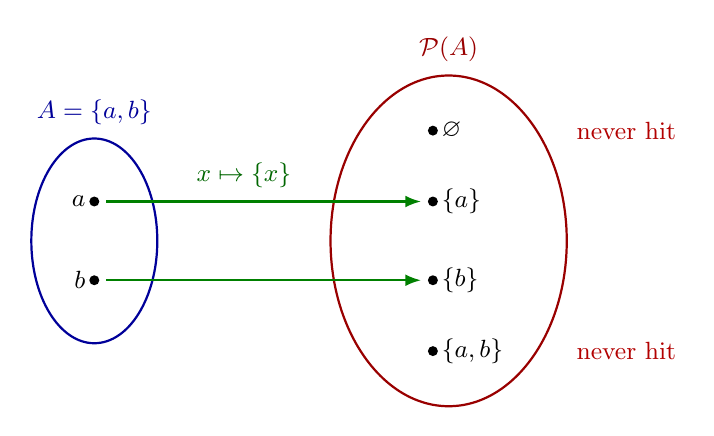
\begin{tikzpicture}[every node/.style={font=\small}, >={Latex[length=2mm]}]
	\draw[thick, blue!60!black] (0,0) ellipse (0.8 and 1.3);
	\node[blue!60!black, anchor=south] at (0,1.35) {$A=\{a,b\}$};
	\fill (0,0.5) circle (1.8pt) node[left, inner sep=3pt] {$a$};
	\fill (0,-0.5) circle (1.8pt) node[left, inner sep=3pt] {$b$};
	\draw[thick, red!60!black] (4.5,0) ellipse (1.5 and 2.1);
	\node[red!60!black, anchor=south] at (4.5,2.15) {$\mathcal{P}(A)$};
	\fill (4.3,1.4) circle (1.8pt) node[right, inner sep=3pt] {$\varnothing$};
	\fill (4.3,0.5) circle (1.8pt) node[right, inner sep=3pt] {$\{a\}$};
	\fill (4.3,-0.5) circle (1.8pt) node[right, inner sep=3pt] {$\{b\}$};
	\fill (4.3,-1.4) circle (1.8pt) node[right, inner sep=3pt] {$\{a,b\}$};
	\draw[->, green!50!black, thick] (0.15,0.5) -- (4.15,0.5);
	\draw[->, green!50!black, thick] (0.15,-0.5) -- (4.15,-0.5);
	\node[green!40!black, font=\small, anchor=south] at (1.9,0.55) {$x\mapsto\{x\}$};
	\node[red!70!black, font=\small, anchor=west] at (6.0,1.4) {never hit};
	\node[red!70!black, font=\small, anchor=west] at (6.0,-1.4) {never hit};
\end{tikzpicture}
\end{document}
